\section{Method}
\label{sec:method}
Place recognition is posed as retrieval: given a query image, we search a database $\mathcal{D}$ of geo-tagged images and return the place of the best match. Scoring every candidate patch by patch is too slow on a database of millions, so we proceed in two stages. We first retrieve and shortlist a fixed number of candidates using a single global descriptor per image, obtained by weighted second-order pooling of its patch features. We then re-rank that shortlist by explicit patch-to-patch \textsc{MaxSim} matching. Both stages read similarities between patch features, and one frozen forward pass per image supplies them.

\begin{figure}[t]
\centering
% \resizebox{\textwidth}{!}{\begin{tikzpicture}[
  font=\small, text=ink, >=Stealth,
  box/.style={draw=ink!35, fill=greyb, rounded corners=2pt, align=center,
    inner sep=4.5pt, minimum height=9mm, font=\small},
  shbox/.style={draw=accent, line width=1pt, fill=accbg, rounded corners=2pt,
    align=center, inner sep=5pt, font=\small},
  s1box/.style={draw=sone!65, line width=0.7pt, fill=sonebg, rounded corners=2pt,
    align=center, inner sep=4.5pt, minimum height=11mm, font=\small},
  s2box/.style={draw=stwo!70, line width=0.7pt, fill=stwobg, rounded corners=2pt,
    align=center, inner sep=4.5pt, minimum height=11mm, font=\small},
  ar/.style={-{Stealth[length=5pt]}, draw=ink!65, line width=0.6pt},
  accar/.style={-{Stealth[length=5pt]}, draw=accent, line width=1pt, dashed},
  dimlbl/.style={font=\scriptsize, text=ink!60, fill=white, inner sep=1pt},
  lbl/.style={font=\scriptsize\itshape, text=ink!70},
  note/.style={font=\scriptsize, text=ink!75, align=center},
]

% ================= INPUT IMAGE + PATCH GRID =================
\node[draw=ink!45, fill=blue!4, minimum width=17mm, minimum height=15mm,
      inner sep=0, rounded corners=1pt] (imgN) at (0,0) {};
\draw[fill=ink!12, draw=ink!35, line width=0.4pt] ($(imgN.south west)+(2pt,0)$) rectangle ($(imgN.south west)+(6pt,9pt)$);
\draw[fill=ink!18, draw=ink!35, line width=0.4pt] ($(imgN.south west)+(6pt,0)$) rectangle ($(imgN.south west)+(11pt,13pt)$);
\draw[fill=ink!12, draw=ink!35, line width=0.4pt] ($(imgN.south west)+(11pt,0)$) rectangle ($(imgN.south west)+(15pt,7pt)$);
\foreach \i in {1,...,5}{\draw[accent!45,line width=0.3pt] ($(imgN.south west)+(\i*17/6*1mm,0)$)--($(imgN.north west)+(\i*17/6*1mm,0)$);}
\foreach \j in {1,...,4}{\draw[accent!45,line width=0.3pt] ($(imgN.south west)+(0,\j*3mm)$)--($(imgN.south east)+(0,\j*3mm)$);}
\node[note, below=1pt of imgN] {query / DB image + patch grid};

% ================= FROZEN BACKBONE =================
\node[box, right=7mm of imgN, minimum height=17mm, minimum width=31mm] (bb)
  {\textbf{Frozen ViT}\\[2pt]
   {\scriptsize\begin{tabular}{@{}ll@{}} DINOv2-G & blk 31\\ DINOv3-L & blk 20\\ DINOv3-7B & blk 32\end{tabular}}\\[1pt]
   {\scriptsize value facet $\cdot$ \emph{no gradient}}};
\coordinate (sf) at ($(bb.north east)+(-4pt,-4pt)$);
\foreach \a in {0,60,120}{\draw[accent,line width=0.7pt] ($(sf)+(\a:3.4pt)$)--($(sf)+(\a+180:3.4pt)$);}

% ================= TOKEN SLAB =================
\node[right=9mm of bb, inner sep=0] (tokanchor) {};
\fill[greyb, draw=ink!35, line width=0.5pt] ($(tokanchor.center)+(-4pt,4pt)$) rectangle ($(tokanchor.center)+(14pt,20pt)$);
\fill[white, draw=ink!35, line width=0.5pt] ($(tokanchor.center)+(0,0)$) rectangle ($(tokanchor.center)+(18pt,16pt)$);
\foreach \k in {1,2,3}{\draw[ink!20,line width=0.3pt] ($(tokanchor.center)+(0,\k*4pt)$) -- ($(tokanchor.center)+(18pt,\k*4pt)$);}
\node[dimlbl, anchor=south] at ($(tokanchor.center)+(7pt,25pt)$) {patch tokens $F$, $N{\times}C$};
\node[note, text=ink!60, anchor=north] (tokdims) at ($(tokanchor.center)+(7pt,-8pt)$)
  {\scriptsize G $2401{\times}1536$\\ L $2304{\times}1024$\\ 7B $2304{\times}4096$};

\draw[ar] (imgN) -- (bb);
\draw[ar] (bb) -- ($(tokanchor.center)+(-6pt,8pt)$);

% ================= SHARED OPS =================
\node[shbox, right=11mm of tokanchor, minimum width=35mm] (sh)
  {\textbf{shared read-invariant ops}\\[3pt]
   \begin{tabular}{@{}l@{}}
   $\bullet$ token-PCA $\;C\!\to\!1024$ \;{\scriptsize(300 unlabelled DB imgs)}\\[3pt]
   $\bullet$ burst weight $w_p=1/d_p$\\
   \quad{\scriptsize $d_p=\#\{p'\!:\langle f_p,f_{p'}\rangle>\tau\}$ --- thresholded, not a raw row-sum}
   \end{tabular}};
\draw[ar] ($(tokanchor.center)+(9pt,8pt)$) -- (sh);

% ================= STAGE 1 (TOP) =================
\node[s1box, minimum width=28mm, anchor=west] (c1) at ($(sh.east)+(3.0,3.4)$)
  {assign to $K{=}32$ cells\\[1pt] {\scriptsize $k$-means on 300}\\ {\scriptsize unlabelled DB images}};
\node[s1box, right=7mm of c1, minimum width=25mm] (c2)
  {burst-weighted residual\\ sums $+$ power law\\ {\scriptsize $\rho(v)\!=\!\mathrm{sign}(v)\sqrt{|v|}$}};
\node[s1box, right=7mm of c2, minimum width=28mm] (c3)
  {desc-PCA $\to 1024$\\ {\scriptsize $\sim$2\,KB $\cdot$ $32\times$ smaller}\\ {\scriptsize costs $0.3$--$3.7$ R@100$^\dagger$}};
\node[s1box, right=7mm of c3, minimum width=27mm] (c4)
  {inner-product scan\\ \emph{whole database}\\ {\scriptsize $\to$ top-$K$ shortlist}};
\draw[ar] (c1) -- (c2);
\draw[ar] (c2) -- node[dimlbl,above]{$32768$} (c3);
\draw[ar] (c3) -- node[dimlbl,above]{$1024$} (c4);

\coordinate (bandmid) at ($(c1.west)!0.5!(c4.east)$);
\node[anchor=west, font=\footnotesize\bfseries, text=sone] at (c1.west |- 0,4.75)
  {Stage 1 $\cdot$ coarse retrieval \textnormal{\scriptsize(polynomial kernel $\Rightarrow$ decomposable)}};
\node[anchor=north, note, draw=ink!25, fill=white, rounded corners=2pt, inner sep=3pt]
  at (bandmid |- 0,2.05)
  {\scriptsize top-$K$ = 100 (Pitts) $\cdot$ 1000 (Tokyo, MSLS, SF, Nordland) $\cdot$ full DB (AmsterTime)};

% ================= STAGE 2 (BOTTOM) =================
% MaxSim mini visual (zero-size anchor at its left)
\coordinate (mm) at ($(sh.east)+(3.15,-3.4)$);
\foreach \i in {0,1,2}\foreach \j in {0,1,2}{\fill[sonebg,draw=sone!50,line width=0.3pt] ($(mm)+(\i*3.5pt,\j*3.5pt)$) rectangle ($(mm)+(\i*3.5pt+3.5pt,\j*3.5pt+3.5pt)$);}
\foreach \i in {0,1,2}\foreach \j in {0,1,2}{\fill[stwobg,draw=stwo!50,line width=0.3pt] ($(mm)+(30pt+\i*3.5pt,\j*3.5pt)$) rectangle ($(mm)+(30pt+\i*3.5pt+3.5pt,\j*3.5pt+3.5pt)$);}
\draw[stwo,line width=0.5pt,-{Stealth[length=3pt]}] ($(mm)+(9pt,9pt)$) -- ($(mm)+(31pt,5pt)$);
\draw[stwo,line width=0.5pt,-{Stealth[length=3pt]}] ($(mm)+(9pt,2pt)$) -- ($(mm)+(35pt,9pt)$);
\draw[stwo,line width=0.5pt,-{Stealth[length=3pt]}] ($(mm)+(5pt,5pt)$) -- ($(mm)+(37pt,2pt)$);
\node[note, text=ink!60, anchor=north] at ($(mm)+(20pt,-3pt)$) {\scriptsize query $\to$ candidate\\[-1pt]\scriptsize max-sim patch};
\node[note, text=sone, anchor=south, font=\scriptsize] at ($(mm)+(5pt,12pt)$) {query};
\node[note, text=stwo, anchor=south, font=\scriptsize] at ($(mm)+(35pt,12pt)$) {cand.};

\node[s2box, minimum width=44mm, anchor=west] (r2) at ($(mm)+(58pt,0)$)
  {weighted \textsc{MaxSim} $+$ confidence gate\\[2pt]
   $\displaystyle \mathrm{score}=\sum_i w_i\,\big[\max_j\langle a_i,b_j\rangle>\tau\big]\max_j\langle a_i,b_j\rangle$\\[2pt]
   {\scriptsize gate: keep the term only if $\max_j\langle a_i,b_j\rangle>0.65$}};
\node[s2box, right=7mm of r2, minimum width=24mm] (r3)
  {re-ranked list\\ {\scriptsize $\to$ R@1 / R@5 / R@10}};
\draw[ar] ($(mm)+(40pt,4pt)$) -- (r2);
\draw[ar] (r2) -- (r3);

\node[anchor=west, font=\footnotesize\bfseries, text=stwo] at (c1.west |- 0,-1.95)
  {Stage 2 $\cdot$ re-ranking \textnormal{\scriptsize(per-row max $\Rightarrow$ never decomposable)}};

% 说明:原本这里有一个 "optional (AmsterTime only) ZCA whitening" 方框,已删除 ——
% 那是逐数据集开关,与 \S\ref{sec:transfer} 主张的"没有逐集开关"直接冲突。
\node[draw=stwo!55, dashed, rounded corners=2pt, fill=stwobg!40, inner sep=5pt,
      font=\scriptsize, align=left, text=ink!80, anchor=north] (zca) at (r2.south |- 0,-5.0)
  {$\diamond$\; \textbf{one configuration everywhere}\\
   same layer, same $\tau$, same threshold, same $K$ --- no per-dataset switch};

% ================= SHARED (two reads) ARROWS =================
\draw[accar] (sh.north) to[out=90,in=180] node[lbl,above,pos=0.5]{read 1: first-order pooling (VLAD)} (c1.west);
\draw[accar] (sh.south) to[out=-90,in=180] node[lbl,below,pos=0.5]{read 2: per-token late interaction} ($(mm)+(-4pt,4pt)$);
\draw[ar] (c4.south) to[out=-90,in=90] node[lbl,right,pos=0.4]{top-$K$ candidates} (r2.north);

% ================= STORAGE + FOOTNOTE =================
\node[anchor=west, draw=store!55, dashed, rounded corners=2pt, inner sep=5pt,
      font=\scriptsize, align=left, text=store] (stor) at (imgN.west |- 0,-6.5)
  {\textbf{STORED / image:}\;\; global descriptor $1024$-d $\approx$ \textbf{2\,KB} (scans full DB) \;\;$|$\;\;
   weighted tokens $512{\times}512\approx$ \textbf{0.52\,MB} (only the shortlist is re-ranked)};
\node[anchor=east, note, text=ink!55] at (c4.east |- 0,-6.5)
  {\scriptsize $^\dagger$ $0.3$ R@100 on databases below $10^4$ images, $2.6$--$3.7$ above; ordering vs.\ second order is unchanged};

% ================= TITLE =================
\node[anchor=south west, font=\large\bfseries, text=ink] at (imgN.west |- 0,2.55)
  {One frozen forward, one weight, two reductions
   \textnormal{\normalfont\small--- no VPR training, no place labels}};

% ================= BANDS =================
\begin{scope}[on background layer]
  \node[fill=sonebg!45, rounded corners=4pt, fit=(c1)(c4), inner sep=7pt] {};
  \coordinate (mmA) at ($(mm)+(-4pt,14pt)$);
  \coordinate (mmB) at ($(mm)+(40pt,-16pt)$);
  \node[fill=stwobg!45, rounded corners=4pt, fit=(mmA)(mmB)(r3)(zca), inner sep=7pt] {};
\end{scope}

\end{tikzpicture}
}  % TikZ version, swapped out for a trial
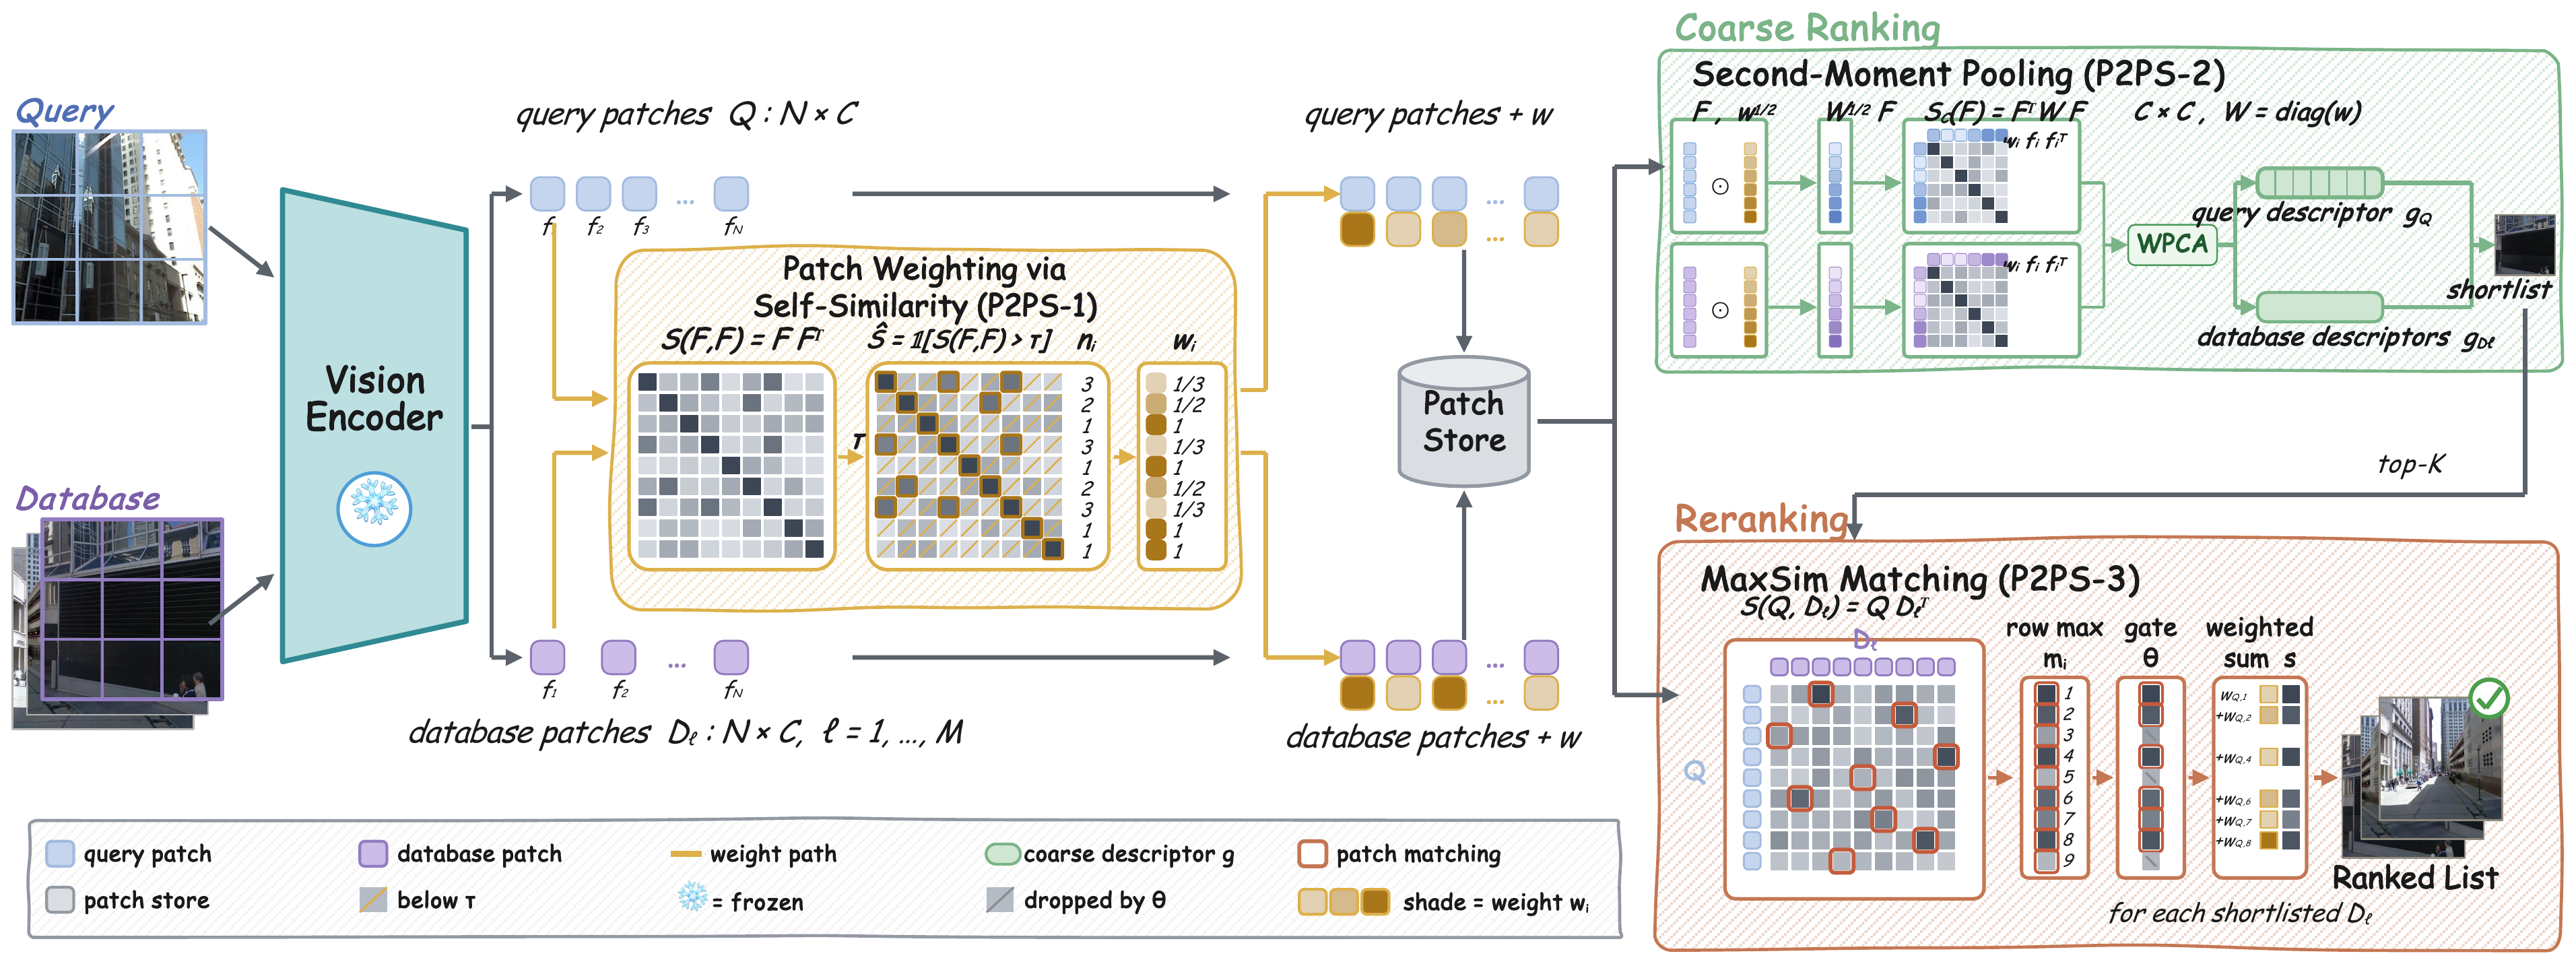
\includegraphics[width=\textwidth]{figures/method_fig_ppt.png}
\caption{\textbf{One frozen forward, one weight, two reductions.} Thresholding and row-summing $G_N{=}FF^{\top}$ gives $w_i{=}1/n_i$, which weights both stages and prunes the store. Stage 1 scans the whitened second moment $G_C{=}F^{\top}WF$; stage 2 re-ranks its shortlist by the row-max reduction of $S{=}QD^{\top}$.}
\label{fig:method}
\end{figure}

\subsection{Tokens}
\label{sec:prelim}
An image is passed through a frozen DINOv2/DINOv3 backbone, and we take the value facet of a fixed block, the output of its value projection, which \citet{vitfacets} introduced as a dense descriptor and \citet{effovpr} adopted for VPR. A PCA is fitted across patch tokens collected from a few hundred unlabelled database images and is then applied to every token, reducing it to $C{=}512$ channels; each token is $\ell_2$-normalized before and after. This gives $N$ unit-norm patch features per image, written $\mathbf f_1,\dots,\mathbf f_N$ and stacked row-wise as $F$. Two kinds of similarity follow: within one image, $G_{ij}=\mathbf f_i^{\top}\mathbf f_j$, and between a query and a candidate, $S_{ij}=\mathbf q_i^{\top}\mathbf d_j$. Block, facet and shortlist depth are swept in Appendix~\ref{app:hyper}.

\subsection{The weight}
\label{sec:feat}
A patch of sky, or one window in a facade of identical windows, appears many times in the same image, and every copy is counted again. We want ten nearly identical sky patches to contribute about as much as one unique patch, rather than ten times as much. We therefore give each patch a weight before either stage uses it.

For token $i$, we want the total weight of the tokens similar to it to be approximately constant. If $G_{ij}$ measures token similarity, this condition reads
\begin{equation}\label{eq:demo}
  \sum_j G_{ij}\,w_j = 1,
  \qquad\text{or in matrix form}\qquad
  G\mathbf w=\mathbf 1,
\end{equation}
which is the democratic-weighting condition of \citet{democratic} and \citet{gmp}. We impose it not on $G$ but on its thresholded version $\hat G_{ij}=\mathbb 1[\,G_{ij}>\tau\,]$, which counts near-duplicates instead of grading them. The condition then has a closed-form solution,
\begin{equation}\label{eq:weight}
  w_i=\frac{1}{n_i},
  \qquad
  n_i=\sum_j \hat G_{ij},
\end{equation}
the reciprocal of the number of patches in the image that resemble patch $i$: a sky patch that appears twenty times receives one twentieth of the weight of a patch that appears once. Appendix~\ref{app:ridge} derives this and relates it to the regularized solution of \citet{gmp}. The only constant is the threshold $\tau$, fixed at $0.5$ for every backbone and dataset. Figure~\ref{fig:vis-c1} draws the near-duplicate groups at that threshold.

\subsection{First stage}
\label{sec:global}
Stage 1 needs a fixed-size descriptor for each image so that all database images can be searched efficiently. We obtain it by weighted second-order pooling of the patch features.

Take one patch $\mathbf q$ from the query and one patch $\mathbf d$ from a candidate. Their similarity is $\mathbf q^{\top}\mathbf d$, and its square can be rewritten as $(\mathbf q^{\top}\mathbf d)^2=\langle\,\mathbf q\mathbf q^{\top},\ \mathbf d\mathbf d^{\top}\,\rangle$, a comparison of two matrices, each built from one image alone. Summing over all patch pairs with the weights of \S\ref{sec:feat} therefore separates into a single comparison between two per-image matrices,
\begin{equation}\label{eq:so-deriv}
  \sum_{i,j} w_{Q,i}\,w_{D,j}\,\big(\mathbf q_i^{\top}\mathbf d_j\big)^{2}
  =\big\langle\, G_C(Q),\ G_C(D)\,\big\rangle,
  \qquad
  G_C(F)=\frac{1}{\sum_i w_i}\sum_i w_i\,\mathbf f_i\mathbf f_i^{\top}.
\end{equation}
$G_C$ records how the image's features co-occur across channels, with no reference to where in the image they appeared, which is what lets two views of a place match under a change of viewpoint, and it retains far more than an average of the features would (Appendix~\ref{app:coarsegrid}). Other powers of the similarity factorize in the same way, as Appendix~\ref{app:factorize} works out.

The stored descriptor is $G_C$ flattened, with a square root applied to each entry, and the result $\ell_2$-normalized:
\begin{equation}\label{eq:stage1}
  \psi(F)\;=\;\frac{\rho\big(\operatorname{vec}(G_C(F))\big)}{\lVert\rho\big(\operatorname{vec}(G_C(F))\big)\rVert_2},
  \qquad
  \rho(u)=\operatorname{sign}(u)\sqrt{|u|}.
\end{equation}
The square root is the power normalization of \citet{improvedfisher}, standard for Fisher vectors and VLAD \citep{allvlad}. Its purpose is the same as the weight's. A repeated element makes a few entries of the descriptor very large, and those entries then dominate the comparison between two images. Taking square roots pulls the large entries down and lets the rest of the descriptor count. The weight acts on patches before pooling and the square root acts on the descriptor after it, so the two do not overlap.

The descriptor is reduced to $2048$ dimensions by a whitened PCA, again fitted on the deployment database, and the scan returns the $P{=}\min(1000,|\mathcal{D}|)$ best candidates. The same weight also decides what to store: each image keeps its $1024$ highest-weight patches, with the weights computed on the full set and carried along (\S\ref{sec:stage1abl}). Nothing is fitted outside $\mathcal{D}$; Figure~\ref{fig:patchcov} shows the stored matrix.

\subsection{Second stage}
\label{sec:core}
For each query patch we find its most similar patch in the candidate image and sum those similarities,
\begin{equation}\label{eq:stage2}
  s(Q,D)=\sum_{i=1}^{N_Q} w_{Q,i}\;\mathbb 1[\,m_i>\theta\,]\;m_i
  \qquad\text{with}\qquad
  m_i=\max_{j} S_{ij},
\end{equation}
which is the \textsc{MaxSim} late-interaction rule of \citet{colbert}, weighted as in \S\ref{sec:feat}. Sky, pedestrians and occluders have no counterpart in the other image, and \textsc{MaxSim} would still score them at their best accidental match, so a patch counts only if its best match clears a confidence threshold $\theta$, fixed at $0.65$ throughout; Appendix~\ref{app:calib} gives the sweep and the reasoning behind it.

Unlike the first stage, \textsc{MaxSim} cannot be represented by a single fixed-size image descriptor, so we apply it only to the shortlisted candidates, which keeps it affordable; Appendix~\ref{app:nofactor} explains why no such descriptor exists. A method that stores one descriptor per image is therefore denied this stage, and must train its pooling until that single vector separates places on its own \citep{netvlad}. The tables denote our rule \textsc{selfw\_conf}, and Figure~\ref{fig:vis-m1} draws its surviving matches. A variant \textsc{mnn\_selfw65} additionally requires each match to be mutual and counts weighted inliers instead of summing similarities; Appendix~\ref{app:effo-matched} runs both against \textsc{EffoVPR}'s attention-selected rule on an identical shortlist and identical features.
